\section{Learning the weight sharing scheme}
\label{sec:learningscheme}

\subsection{Discussion}

In the ternary representation $Y = h(\wideparen{\Theta S X})$ of a layer~$\cl$, the weight kernel~$\Theta$ is usually the only operand that is learned, and the role of~$S$ is to label the edges of the propagation graph~$P$ with these weights. Recall that, as noted after \defref{def:ter}, $S$ needs not be sparse and composed of one-hot vectors. In that case, the labelling is done linearly as depicted previously in \figref{fig:ternary}. Therefore, the weight sharing scheme $S$ can also be updated during the learning phase. This can be interpreted as learning a convolution-like operator on the underlying graph~$G$~\citep{vialatte2017learning}.

\begin{remark}
When $S$ does not have the sparse priors mentioned in \secref{sec:sparse}, we must not have more parameters in $S$ and $\Theta$ than in $W$, so that the weight sharing still makes sense. If we call $l$ the number of edges in the resulting propagation graph $P$, then the former assumption requires $l\omega + \omega NM \leq lNM$ or equivalently $\frac{1}{\omega} \geq \frac{1}{NM} + \frac{1}{l}$. It implies that the number of weights per filter $\omega$ must be lower than the total number of filters $NM$ and than the number of edges $l$, which is always the case in practice.
\end{remark}

%However, as learning $S$ will require in most cases to lose the sparse priors, this can lead to memory issues and increased time execution. Hence, our first experiments focus on shallow architectures to study feasability. Despite these limitations, the observations could still be useful to understand better the extent of the ternary representation. Nonetheless, these experiments can also see application in deep settings: an approach would be to pick a weight sharing scheme $S$ learned in shallow settings and to share it among ternary representations of convolutional layers of a deep architecture.

%\todo{drop conditional if experiment is done}

\subsection{Experimental settings}
In our experiments, we learn the scheme $S$ and the kernel $\Theta$ simultaneously.

\paragraph{Constraints for supervised classification of graph signals}

Because of our inspiration from CNNs, we propose constraints on the parameters of $S$. Namely, we impose them to be between~$0$ and~$1$, and to sum to~$1$ along the first rank (the rank that is contracted in the product~$\Theta S$).
\begin{gather}
\forall (k,i,j),~S[k,i,j] \in [0,1]\\
\forall (i,j),~\displaystyle \sum_{k=1}^\omega S[k,i,j] = 1
\end{gather}

Therefore, the vectors on the first rank of $S$ can be interpreted as performing a positive weighted average of the parameters in $\Theta$.
Also, we choose to aim our study at graph signals. Hence, we consider a graph $\gve$ and that the layer is EC. For this reason, \propref{prop:aw} tells us that the connectivity matrix~$W$ of the layer is masked by the adjacency matrix~$A$. Therefore, $S$ is also masked by~$A$ \ie we impose the constraint that
\begin{gather}
A[i,j] = 0 \Rightarrow \forall k, S[k,i,j] = 0
\end{gather}

\paragraph{Constraints for semi-supervised classification of nodes}

For the case of citation networks, we consider only one graph and thus we set $\omega = 1$ so that $S$ and $\Theta$ are matrices. Additionaly, we impose rows of the scheme $S$ to be normalized so that each node receives a normalized information from its neighborhood. In our experiments, we choose to use softmax normalization because it is of standard usage (but other normalizations could do as well).

\paragraph{Name}
In \citep{vialatte2017learning}, we used the term \emph{Local Receptive Graph layers}, since \propref{prop:lrf} relates $G$ with local receptive fields defined by $W$. However it was cumbersome so in this manuscript we will just call them \emph{Graph Contraction Layer} in reference to the neural contraction (see \defref{def:ter}). We call \emph{Graph Contraction Networks} (GCT) the corresponding neural networks. The main addition to the paper \citep{vialatte2017learning} from \secref{sec:learningscheme} is \secref{sec:lss}.

\paragraph{Initialization}
In supervised settings, we introduce three types of initialization for the scheme $S$. The last two have the sparse priors mentioned in \secref{sec:sparse}:
\begin{enumerate}
  \item uniform random: parameters of $S$ are simply initialized with a uniform random distribution with limits as described by \cite{glorot2010understanding}.
  \item random one-hot: one-hot vectors are distributed randomly on the $S[:,i,j]$, with the constraint that for each LRF, a particular one-hot vector can only be distributed at most once more than any other.
  \item circulant one-hot: one-hot vectors are distributed in a circulant fashion on the $S[:,i,j]$, so that on Euclidean domains, the initial state of $S$ correspond exactly to the weight sharing scheme of a standard convolution.
\end{enumerate}

In semi-supervised settings, we initialize the scheme $S$ using the normalized adjacency matrix $\widetilde{A}$ to which we add a gaussian noise $\cn(0,\sigma)$, where the standard deviation $\sigma$ is determined following \cite{glorot2010understanding}.

\subsection{Experiments with grid graphs}

We experiment GCTs on the MNIST dataset (see \secref{sec:datasets}). We use a shallow architecture made of a single ternary layer with 50 feature maps, without pooling, followed by a FC layer of 300 neurons, 50\% dropout, and terminated by a FC layer of 10 neurons with softmax activation. ReLu activations are used. Input layers are regularized by a factor weight of $10^{-5}$~\citep{ng2004feature}. We optimize with ADAM~\citep{kingma2014adam} up to 100 epochs and fine-tune (while $S$ is frozen) for up to 50 additional epochs.

For the underlying graph strucure, we consider a grid graph that connects each pixel to itself and its 4 nearest neighbors (or less on the borders). We also consider the square of this graph (pixels are connected to their 13 nearest neighbors, including themselves), the cube of this graph (25 nearest neighbors), up to 10 powers (211 nearest neighbors).
We test the model under two setups: either the ordering of the node is unknown, and then we use random one-hot intialization for $S$; either an ordering of the node is known, and then we use circulant one-hot intialization for $S$ which we freeze in this state. We use the number of nearest neighbors as for the dimension of the first rank of $S$.
We also compare with a convolutional layer of size 5x5, thus containing as many weights as the cube of the grid graph. On MNIST, training architectures that learn $S$ took about twice longer. Table~\ref{toy} summarizes the obtained results. The ordering is unknown for the first result given, and known for the second result between parenthesis.

\begin{table}[H]
  \caption{Error rates (in \%) on powers of the grid graphs on MNIST.}
  \begin{center}
    \bgroup
    \def\arraystretch{1.5}%  1 is the default, change whatever you need
    \begin{tabular}{|c|c|c|c|}
      \hline
      Conv5x5 & Grid$^1$ & Grid$^2$ & Grid$^3$\\
      \hline
      $(0.87)$ & $1.24 (1.21)$ & $1.02 (0.91)$ & $0.93 (0.91)$\\
      \hline
      \hline
      Grid$^4$ & Grid$^5$ & Grid$^6$ & Grid$^{10}$\\
      \hline
      $0.90 (0.87)$ & $0.93 (0.80)$ & $1.00 (0.74)$ & $0.93 (0.84)$\\
      \hline
    \end{tabular}
    \egroup
  \end{center}
  \label{toy}
\end{table}

We observe that even without knowledge of the underlying Euclidean structure, grid GCTs obtain comparable performances as CNNs, and when the ordering is known, they match them. We also noticed that after training, even though the one-hot vectors used for initialization had changed to floating point values, their most significant dimension was almost always the same. That suggests there is room to improve the initialization and the optimization.

In Figure~\ref{functionofepoch}, we plot the test error rate for various normalizations when using the square of the grid graph, as a function of the number of epochs of training, only to find that they have little influence on the performance but sometimes improve it a bit. Thus, we will treat them as optional hyperparameters.

\begin{figure}[H]
  \begin{center}
    % GNUPLOT: LaTeX picture with Postscript
\begingroup
  \makeatletter
  \providecommand\color[2][]{%
    \GenericError{(gnuplot) \space\space\space\@spaces}{%
      Package color not loaded in conjunction with
      terminal option `colourtext'%
    }{See the gnuplot documentation for explanation.%
    }{Either use 'blacktext' in gnuplot or load the package
      color.sty in LaTeX.}%
    \renewcommand\color[2][]{}%
  }%
  \providecommand\includegraphics[2][]{%
    \GenericError{(gnuplot) \space\space\space\@spaces}{%
      Package graphicx or graphics not loaded%
    }{See the gnuplot documentation for explanation.%
    }{The gnuplot epslatex terminal needs graphicx.sty or graphics.sty.}%
    \renewcommand\includegraphics[2][]{}%
  }%
  \providecommand\rotatebox[2]{#2}%
  \@ifundefined{ifGPcolor}{%
    \newif\ifGPcolor
    \GPcolortrue
  }{}%
  \@ifundefined{ifGPblacktext}{%
    \newif\ifGPblacktext
    \GPblacktextfalse
  }{}%
  % define a \g@addto@macro without @ in the name:
  \let\gplgaddtomacro\g@addto@macro
  % define empty templates for all commands taking text:
  \gdef\gplbacktext{}%
  \gdef\gplfronttext{}%
  \makeatother
  \ifGPblacktext
    % no textcolor at all
    \def\colorrgb#1{}%
    \def\colorgray#1{}%
  \else
    % gray or color?
    \ifGPcolor
      \def\colorrgb#1{\color[rgb]{#1}}%
      \def\colorgray#1{\color[gray]{#1}}%
      \expandafter\def\csname LTw\endcsname{\color{white}}%
      \expandafter\def\csname LTb\endcsname{\color{black}}%
      \expandafter\def\csname LTa\endcsname{\color{black}}%
      \expandafter\def\csname LT0\endcsname{\color[rgb]{1,0,0}}%
      \expandafter\def\csname LT1\endcsname{\color[rgb]{0,1,0}}%
      \expandafter\def\csname LT2\endcsname{\color[rgb]{0,0,1}}%
      \expandafter\def\csname LT3\endcsname{\color[rgb]{1,0,1}}%
      \expandafter\def\csname LT4\endcsname{\color[rgb]{0,1,1}}%
      \expandafter\def\csname LT5\endcsname{\color[rgb]{1,1,0}}%
      \expandafter\def\csname LT6\endcsname{\color[rgb]{0,0,0}}%
      \expandafter\def\csname LT7\endcsname{\color[rgb]{1,0.3,0}}%
      \expandafter\def\csname LT8\endcsname{\color[rgb]{0.5,0.5,0.5}}%
    \else
      % gray
      \def\colorrgb#1{\color{black}}%
      \def\colorgray#1{\color[gray]{#1}}%
      \expandafter\def\csname LTw\endcsname{\color{white}}%
      \expandafter\def\csname LTb\endcsname{\color{black}}%
      \expandafter\def\csname LTa\endcsname{\color{black}}%
      \expandafter\def\csname LT0\endcsname{\color{black}}%
      \expandafter\def\csname LT1\endcsname{\color{black}}%
      \expandafter\def\csname LT2\endcsname{\color{black}}%
      \expandafter\def\csname LT3\endcsname{\color{black}}%
      \expandafter\def\csname LT4\endcsname{\color{black}}%
      \expandafter\def\csname LT5\endcsname{\color{black}}%
      \expandafter\def\csname LT6\endcsname{\color{black}}%
      \expandafter\def\csname LT7\endcsname{\color{black}}%
      \expandafter\def\csname LT8\endcsname{\color{black}}%
    \fi
  \fi
    \setlength{\unitlength}{0.0500bp}%
    \ifx\gptboxheight\undefined%
      \newlength{\gptboxheight}%
      \newlength{\gptboxwidth}%
      \newsavebox{\gptboxtext}%
    \fi%
    \setlength{\fboxrule}{0.5pt}%
    \setlength{\fboxsep}{1pt}%
\begin{picture}(5040.00,3528.00)%
    \gplgaddtomacro\gplbacktext{%
      \colorrgb{0.38,0.38,0.38}%
      \put(946,751){\makebox(0,0)[r]{\strut{}$0.01$}}%
      \colorrgb{0.38,0.38,0.38}%
      \put(946,3263){\makebox(0,0)[r]{\strut{}$0.1$}}%
      \colorrgb{0.38,0.38,0.38}%
      \put(1125,484){\makebox(0,0){\strut{}$0$}}%
      \colorrgb{0.38,0.38,0.38}%
      \put(1829,484){\makebox(0,0){\strut{}$20$}}%
      \colorrgb{0.38,0.38,0.38}%
      \put(2532,484){\makebox(0,0){\strut{}$40$}}%
      \colorrgb{0.38,0.38,0.38}%
      \put(3236,484){\makebox(0,0){\strut{}$60$}}%
      \colorrgb{0.38,0.38,0.38}%
      \put(3939,484){\makebox(0,0){\strut{}$80$}}%
      \colorrgb{0.38,0.38,0.38}%
      \put(4643,484){\makebox(0,0){\strut{}$100$}}%
    }%
    \gplgaddtomacro\gplfronttext{%
      \csname LTb\endcsname%
      \put(176,2007){\rotatebox{-270}{\makebox(0,0){\strut{}Test error rate}}}%
      \put(2884,154){\makebox(0,0){\strut{}Epoch}}%
      \csname LTb\endcsname%
      \put(3656,3090){\makebox(0,0)[r]{\strut{}l2}}%
      \csname LTb\endcsname%
      \put(3656,2870){\makebox(0,0)[r]{\strut{}l2 + Pos}}%
      \csname LTb\endcsname%
      \put(3656,2650){\makebox(0,0)[r]{\strut{}None}}%
      \csname LTb\endcsname%
      \put(3656,2430){\makebox(0,0)[r]{\strut{}Norm + Pos}}%
      \csname LTb\endcsname%
      \put(3656,2210){\makebox(0,0)[r]{\strut{}l2 + Pos + Norm}}%
    }%
    \gplbacktext
    \put(0,0){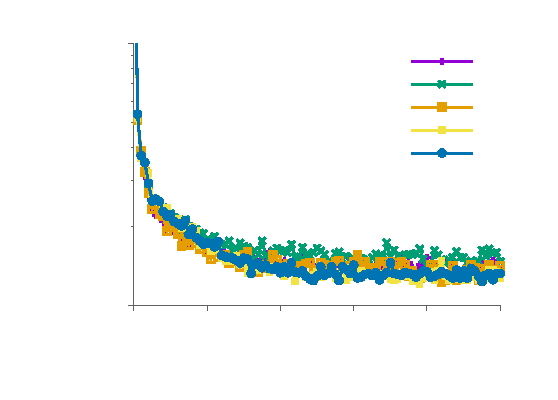
\includegraphics{chapter3/functionofepoch}}%
    \gplfronttext
  \end{picture}%
\endgroup

  \end{center}
  \caption{Evolution of the test error rate when learning MNIST using the square of a grid graph and for various normalizations, as a function of the epoch of training. The legend reads: ``l2'' means $\ell_2$ normalization of weights is used (with weights $10^{-5}$), ``Pos'' means parameters in $S$ are forced to being positive, and ``Norm'' means that the $\ell_1$ norm of each vector in the first dimension of $S$ is forced to 1.}
  \label{functionofepoch}
\end{figure}

\subsection{Experiments with covariance graphs}

As underlying graph structure, we use a thresholded covariance matrix obtained by using all the training examples. We choose the threshold so that the number of remaining edges corresponds to a certain density~$p$ (5x5 convolutions correspond approximately to a density of $p=3\%$). We also infer a graph based on the $k$~nearest neighbors of the inverse of the values of this covariance matrix ($k$-NN). The latter two are using no prior about the signal underlying structure. The pixels of the input images are shuffled and the same re-ordering of the pixels is used for every image. Dimension of the first rank of~$S$ is chosen equal to~$k$ and its weights are initialized random uniformly.
GCTs are also compared with models obtained when replacing the first layer by a fully connected or convolutional one. Architecture used is the same as in the previous section. Results are reported on table~\ref{covar}.

\begin{table}[H]
  \caption{Error rates (in \%) on scrambled MNIST.}
  \begin{center}
    \bgroup
    \def\arraystretch{1.5}%  1 is the default, change whatever you need
    \begin{tabular}{|c|c|c|c|}
      \hline
      MLP & Conv5x5 & Thresholded ($p=3\%$) & $k$-NN ($k=25$)\\
      \hline
      $1.44$ & $1.39$ & $1.06$ & $0.96$\\
      \hline
    \end{tabular}
    \egroup
  \end{center}
  \label{covar}
  \end{table}

We observe that GCTs outperform the CNN and the MLP on scrambled MNIST. This is remarkable because that suggests it has been able to exploit information about the underlying structure.

\subsection{Improved convolutions on shallow architectures}

On CIFAR-$10$ (see \secref{sec:datasets}), we made experiments on shallow CNN architectures and replaced convolutions by receptive graphs. We report results on a variant of AlexNet~\citep{krizhevsky2012imagenet} using little distortion on the input that we forked from a tutorial of tensorflow~\citep{tensorflow2015-whitepaper}.
%On CIFAR-$10$, we use a variant of the AlexNet architecture applied on inputs with little distortion~\cite{krizhevsky2012imagenet}, borrowed from a tutorial of tensorflow~\cite{tensorflow2015-whitepaper}.
It is composed of two 5x5 convolutional layers of 64 feature maps, with max pooling and local response normalization~\citep{krizhevsky2012imagenet}, followed by two fully connected layers of 384 and 192 neurons.
On CIFAR-$10$, training architectures that learn $S$ took about $2.5$ times longer.
%We switched each convolutional layer with receptive graph layers, but kept the pooling ones.
We compare two different graph supports: the one obtained by using the underlying graph of a regular 5x5 convolution, and the support of the square of the grid graph. Optimization is done with stochastic gradient descent on 375 epochs where $S$ is freezed on the 125 last ones. Circulant one-hot intialization is used. These are weak classifiers for CIFAR-$10$ but they are enough to analyse the usefulness of the proposed layer.
%Exploring deeper architectures is left for further work.
Experiments are run five times each. Means and standard deviations of accuracies are reported in table~\ref{cifar}. ``Pos'' means parameters in $S$ are forced to being positive, ``Norm'' means that the $\ell_1$ norm of each vector in the third dimension of $S$ is forced to 1, ``Both'' means both constraints are applied, and ``None'' means none are used.

\begin{table}[H]
  \caption{Accuracies (in \%) of shallow networks on CIFAR-$10$.}
  \begin{center}
    \bgroup
    \def\arraystretch{1.5}%  1 is the default, change whatever you need
    \begin{tabular}{|c|c|c|c|c|c|c|}
      \hline
      Support & Learn $S$ & None & Pos & Norm & Both\\
      \hline
      \hline
      Conv5x5 & No & / & / & / & $86.8 \pm 0.2$\\
      \hline
      Conv5x5 & Yes & $87.4 \pm 0.1$ & $87.1 \pm 0.2$ & $87.1 \pm 0.2$ & $87.2 \pm 0.3$\\
      \hline
      Grid$^2$ & Yes & $87.3 \pm 0.2$ & $87.3 \pm 0.1$ & $87.5 \pm 0.1$ & $87.4 \pm 0.1$\\
      \hline
    \end{tabular}
    \egroup
  \end{center}
  \label{cifar}
\end{table}

The GCTs are able to outperform the corresponding CNNs by a small but statistically significant amount in a shallow architecture.

\h{0}\\

Learning the scheme $S$ implies a memory overhead due to the increase in the number of weights of each layer, thus why we limited this experiment to a shallow architecture. An example of strategy to extend this experiment to deeper architectures is to tie the schemes of each layer together, or to reuse a same scheme (previously learned) for all layers.

%\todo{take S, and reuse it on resnet}

\subsection{Learning $S$ for semi-supervised node classification}
\label{sec:lss}

We benchmark multiple graph convolutional methods on citation networks. We refer the reader to \secref{sec:datasets} for a description of the datasets, and to \secref{sec:vert} for a review of the tested models. The models we benchmark are:
\begin{itemize}[nolistsep,noitemsep]
 \item Graph Convolution Network (GCN, \cite{kipf2016semi}),
 \item Graph Attention Network (GAT, \cite{velickovic2017graph}),
 \item Topology Adaptative GCN (TAGCN,  \cite{du2017topology}),
 \item Addition of graph dropout to GCN (GCN*, from \secref{sec:gsexp}),
 \item Graph Contraction Network (GCT, this work).
\end{itemize}

To proceed, we forked the official code repository of \cite{velickovic2017graph}, in order to replicate their environmental setup, from which we implemented the other tested models. This entailed a few differences\footnote{Thanks to Daniel Grattarola for his helpful discussion \url{https://github.com/danielegrattarola/keras-gat/issues/17}.} to be noted between our implementation of GCN and TAGCN from the original ones: a bias is added, the right products $XW$ are computed first and are followed by $50\%$ dropout, and the best model on the validation set is saved to be reused at test time. We also used $50\%$ graph dropout for GAT, TAGCN, and GCT, except on the Pubmed dataset for which we saw that it was detrimental. The inputs of each layer undergo $50\%$ dropout, and the value of graph dropout of GCN* is also $50\%$. Every model is composed of two hidden layers. GAT models uses $8$ heads with $8$ hidden units (which amounts to $64$ hidden units), whereas the number of hidden units for other models was grid searched in $\{16, 32, 64\}$\footnote{Most of the time the value of $16$ was selected, sometimes $32$, and never $64$.}. The polynomial degree of TAGCN was $2$. For comparison, we also ran the experiment with an MLP composed of $500$ hidden neurons. The results are reported in \tabref{tab:lss}.

\begin{table}[H]
\begin{center}
  \bgroup
  \def\arraystretch{1.5}%  1 is the default, change whatever you need
  \begin{tabular}{|c|c|c|c|c|c|c|}
    \hline
    Dataset & MLP & GCN & GAT & TAGCN & GCN* & GCT\\
    \hline
    \hline
    Cora & $58.8 \pm 0.9$ & $81.8 \pm 0.9$ & $83.3 \pm 0.6$ & $82.9 \pm 0.7$ & $\mathbf{83.4} \pm 0.7$ & $83.3 \pm 0.7$\\
    \hline
    Citeseer & $56.7 \pm 1.1$ & $72.2 \pm 0.6$ & $72.1 \pm 0.6$ & $71.7 \pm 0.7$ & $72.5 \pm 0.8$ & $\mathbf{72.7} \pm 0.5$\\
    \hline
    Pubmed & $72.6 \pm 0.9$ & $79.0 \pm 0.5$ & $78.3 \pm 0.7$ & $78.9 \pm 0.5$ & $78.2 \pm 0.7$ & $\mathbf{79.2} \pm 0.4$\\
    \hline
  \end{tabular}
  \egroup
\end{center}
\caption{Mean accuracy (in \%) and standard deviation from 100 runs}
\label{tab:lss}
\end{table}

Even though GCT models performed best overall, the differences with the second bests are not statistically significant. In particular, GCN models enjoy a bump in performances in this setup compared to the experiments in the original paper. The addition of graph dropout put them back on par with the other models on CORA and Citeseer (they were already ahead on Pubmed). We also noticed that the results we obtained for TAGCN on Pubmed were significantly worse than claimed by the authors. We contacted them to check for details and are awaiting response, so we may amend this result in a future version of this document\footnote{However it is possible that this is due to the experimental setup.}. It is worth noting that the MLP performed a lot worse as expected since it did not exploit the graph structure.